\chapter{Conditions d'optimalité}
\label{chap:optimality-conditions}

\section{Introduction et définitions}

\begin{definition}[Ensemble actif]
Soit $x \in \Omega$ un point réalisable. L'ensemble actif (\textit{active set}), noté $\mathcal{A}(x)$, est constitué des indices des contraintes d'égalité et des indices des contraintes d'inégalité qui sont saturées (égales à 0) en $x$.
\[
    \mathcal{A}(x) = \mathcal{E} \cup \{ i \in \mathcal{I} \mid c_i(x) = 0 \}.
\]
\begin{itemize}
    \item Une contrainte $i \in \mathcal{I}$ est dite \textbf{active} si $c_i(x) = 0$ (donc $i \in \mathcal{A}(x)$).
    \item Elle est dite \textbf{inactive} si $c_i(x) > 0$ (donc $i \notin \mathcal{A}(x)$).
\end{itemize}
\end{definition}

\begin{figure}[H]
\centering
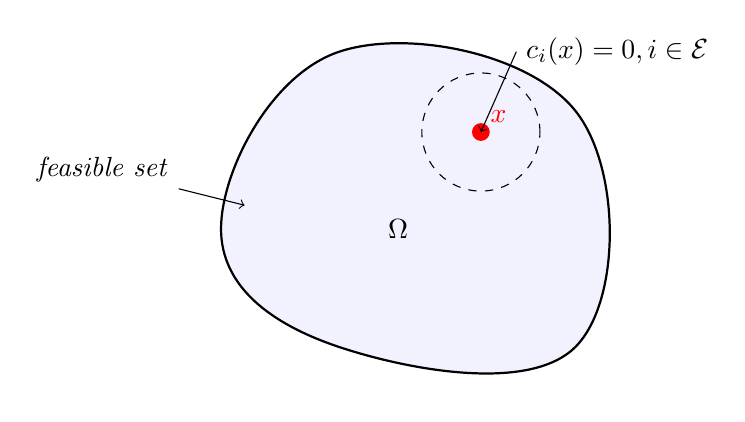
\begin{tikzpicture}[scale=1.5]
    % Draw the feasible set Omega (irregular shape)
    \draw[thick, fill=blue!5] plot [smooth cycle, tension=0.7] coordinates {(-1,0) (0,1.5) (2,1) (2,-1) (0,-1)};
    \node at (0.5, 0) {$\Omega$};
    
    % Draw "feasible set" label with arrow
    \node (feasible) at (-2, 0.5) {\textit{feasible set}};
    \draw[->] (feasible) -- (-0.8, 0.2);
    
    % Draw a point x on the boundary
    \coordinate (x) at (1.2, 0.82); % Approximate boundary point
    \filldraw[red] (x) circle (2pt) node[above right] {$x$};
    
    % Indicate active constraints intersection conceptually
    % Drawing a small circle around x to indicate local inspection
    \draw[dashed] (x) circle (0.5cm);
    
    % Annotations based on the blackboard drawing
    % The drawing shows c_i(x)=0 for active, c_i(x)>0 for inactive inside
    \draw[->] (1.5, 1.5) node[right] {$c_i(x)=0, i \in \mathcal{E}$} -- (x);
    
\end{tikzpicture}
\caption{Illustration de l'ensemble réalisable $\Omega$ et d'un point $x$ sur la frontière où certaines contraintes sont actives.}
\label{fig:active-set}
\end{figure}

\begin{figureexplanation}
\textbf{Interprétation géométrique :}
\begin{itemize}
    \item L'ensemble $\Omega$ est la région réalisable (en bleu).
    \item Le point $x$ est sur la frontière. Les contraintes actives ($c_i(x)=0$) sont celles dont la frontière passe exactement par $x$.
    \item Les autres contraintes (inactives) satisfont $c_i(x) > 0$ et ne limitent pas \emph{localement} les mouvements infinitésimaux autour de $x$.
\end{itemize}
\end{figureexplanation}

\section{Exemples}

\subsection{Une contrainte d'égalité}

Considérons le problème de minimisation suivant dans $\mathbb{R}^2$ :
\begin{equation}
    \min_{(x_1, x_2) \in \mathbb{R}^2} x_1 + x_2 \quad \text{sous la contrainte} \quad x_1^2 + x_2^2 - 2 = 0.
\end{equation}
On a ici :
\begin{align*}
    f(x) &= x_1 + x_2, \\
    c_1(x) &= x_1^2 + x_2^2 - 2, \\
    \mathcal{E} &= \{1\}, \quad \mathcal{I} = \emptyset.
\end{align*}
L'ensemble réalisable est le cercle de centre $(0,0)$ et de rayon $\sqrt{2}$.
Calculons les gradients :
\begin{equation}
    \nabla f(x) = \begin{pmatrix} 1 \\ 1 \end{pmatrix}, \quad \nabla c_1(x) = \begin{pmatrix} 2x_1 \\ 2x_2 \end{pmatrix}.
\end{equation}

On remarque que $\nabla f(x)$ est constant (le même en tout point), contrairement à $\nabla c_1(x)$ qui dépend de la position sur le cercle.

\begin{figure}[H]
\centering
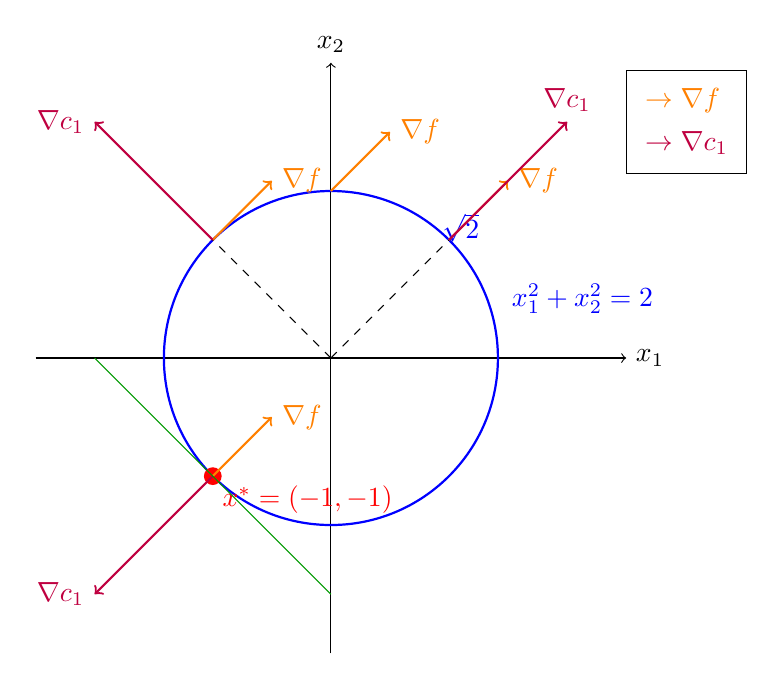
\begin{tikzpicture}[scale=1.5]
    % Axes
    \draw[->] (-2.5,0) -- (2.5,0) node[right] {$x_1$};
    \draw[->] (0,-2.5) -- (0,2.5) node[above] {$x_2$};
    
    % Circle (Feasible set)
    \draw[thick, blue] (0,0) circle (1.414);
    \node[blue] at (1.1, 1.1) {$\sqrt{2}$};
    \node[blue, right] at (1.45, 0.5) {$x_1^2+x_2^2=2$};
    
    % Scaling for visualization: 
    % Real norms: ||grad f|| = sqrt(2) approx 1.414. ||grad c1|| = 2*sqrt(2) approx 2.828.
    % We visually scale them down by factor 0.5 to fit.
    % Visual lengths: grad f -> 0.7 units. grad c1 -> 1.4 units.
    
    % Point 1 (1, 1)
    \coordinate (P1) at (1,1);
    \draw[dashed] (0,0) -- (P1);
    % grad f = (1,1) -> visual (0.5, 0.5)
    \draw[->, orange, thick] (P1) -- ++(0.5, 0.5) node[right] {$\nabla f$};
    % grad c1 = (2,2) -> visual (1, 1) -> 2x larger
    % Shifted slightly to distinguish
    \draw[->, purple, thick] (P1) -- ++(1.0, 1.0) node[above] {$\nabla c_1$};
    
    % Point 2 (-1, 1)
    \coordinate (P2) at (-1,1);
    \draw[dashed] (0,0) -- (P2);
    % grad f = (1,1) -> visual (0.5, 0.5)
    \draw[->, orange, thick] (P2) -- ++(0.5, 0.5) node[right] {$\nabla f$}; 
    % grad c1 = (-2,2) -> visual (-1, 1) -> 2x larger
    \draw[->, purple, thick] (P2) -- ++(-1.0, 1.0) node[left] {$\nabla c_1$};
    
    % Optimal Point (-1, -1)
    \coordinate (Opt) at (-1,-1);
    \filldraw[red] (Opt) circle (2pt);
    \node[red, below right] at (-1, -1) {$x^* = (-1, -1)$};
    
    % Gradients at Opt
    % grad f = (1,1) -> visual (0.5, 0.5)
    \draw[->, orange, thick] (Opt) -- ++(0.5, 0.5) node[right] {$\nabla f$};
    % grad c1 = (-2,-2) -> visual (-1, -1) -> 2x larger
    \draw[->, purple, thick] (Opt) -- ++(-1.0, -1.0) node[left] {$\nabla c_1$};
    
    % Tangent line at Opt (x+y = -2)
    \draw[green!60!black, thin] (-2, 0) -- (0, -2);
    
    % Another point to show "reducing function" idea
    % Intermediate point on circle, e.g., (0, sqrt(2)) ~ (0, 1.414)
    \coordinate (P3) at (0, 1.414);
    % grad f = (1,1) -> visual (0.5, 0.5)
    \draw[->, orange, thick] (P3) -- ++(0.5, 0.5) node[right] {$\nabla f$};
    % grad c1 = (0, 2*sqrt(2)) -> direction (0,1)
    % Just showing f here to unclutter
    
    % Legend
    \matrix [draw, fill=white, right] at (2.5, 2) {
      \node[orange] {$\to \nabla f$}; \\
      \node[purple] {$\to \nabla c_1$}; \\
    };
\end{tikzpicture}
\caption{Minimisation de $x_1+x_2$ sur le cercle. Au point optimal $x^*=(-1,-1)$, les gradients $\nabla f$ et $\nabla c_1$ sont colinéaires et de sens opposés. Notons que $\|\nabla c_1(x)\| = 2\|\nabla f(x)\|$ sur le cercle.}
\label{fig:ex-equality-constraint}
\end{figure}

\begin{figureexplanation}
\textbf{Commentaires :}
\begin{itemize}
    \item \textbf{Variation de la fonction objectif} : Depuis n'importe quel point du cercle (autre que l'optimum), il est possible de se déplacer le long du cercle ("reduce the function while staying on the circle") pour diminuer la valeur de $f$.
    \item \textbf{Comportement des gradients} : Le gradient de la fonction objectif $\nabla f$ est le même en tout point (vecteur constant $(1,1)$), ce qui n'est pas le cas des vecteurs contraintes $\nabla c_1(x)$ qui changent de direction selon le point considéré sur le cercle (vecteurs radiaux).
    \item \textbf{Condition d'optimalité} : À l'optimum $x^*=(-1,-1)$, il n'est plus possible de diminuer $f$ tout en restant sur le cercle. Géométriquement, cela correspond au point où les lignes de niveau de $f$ sont tangentes au cercle. Algébriquement, on observe que $\nabla f(x^*)$ et $\nabla c_1(x^*)$ sont colinéaires.
\end{itemize}
\end{figureexplanation}

\begin{remarque}
Au point $x^* = (-1, -1)$, le gradient de la contrainte $\nabla c_1(x^*) = \begin{pmatrix} -2 \\ -2 \end{pmatrix}$ est parallèle au gradient de la fonction objectif $\nabla f(x^*) = \begin{pmatrix} 1 \\ 1 \end{pmatrix}$.

Il existe un scalaire $\lambda_1^* \in \mathbb{R}$ tel que :
\begin{equation}
    \nabla f(x^*) = \lambda_1^* \nabla c_1(x^*).
\end{equation}
Dans cet exemple, on trouve $\lambda_1^* = -1/2$.
\end{remarque}

\paragraph{Dérivation (Justification heuristique)}
Soit $x$ un point réalisable. Un petit pas $s$ partant de $x$ reste réalisable si, au premier ordre :
\begin{equation}
    0 = c_1(x+s) \approx \underbrace{c_1(x)}_{=0} + \nabla c_1(x)^T s.
\end{equation}
Donc, pour rester sur la surface de contrainte (au premier ordre), le pas $s$ doit être orthogonal au gradient de la contrainte : $\nabla c_1(x)^T s = 0$.

De plus, le pas $s$ produit une diminution de la fonction objectif $f$ si :
\begin{equation}
    0 > f(x+s) - f(x) \approx \nabla f(x)^T s \quad \text{(au premier ordre)}.
\end{equation}
C'est-à-dire $\nabla f(x)^T s < 0$ (pour un pas $s$ suffisamment petit).

Si $x^*$ est un minimum local, il ne doit pas exister de direction $s$ qui soit à la fois réalisable (tangente à la contrainte) et de descente. Cela implique que le gradient $\nabla f(x^*)$ doit être aligné avec $\nabla c_1(x^*)$. Si $\nabla f(x^*)$ avait une composante non nulle dans l'espace tangent, on pourrait trouver un $s$ réduisant $f$.

Cela suggère qu'on cherche une direction $d$ (par exemple avec $\|d\|=1$) telle que :
\begin{equation}
    \begin{cases}
    \nabla c_1(x)^T d = 0 \quad \text{(tangente à la surface)} \\
    \nabla f(x)^T d < 0 \quad \text{(descente)}
    \end{cases}
\end{equation}
S'il n'existe pas de tel $d$, alors il est probable que $x$ soit un minimiseur local.

Cela ne peut être le cas que si $\nabla f(x)$ et $\nabla c_1(x)$ sont parallèles, c'est-à-dire :
\begin{equation}
    \nabla f(x) = \lambda_1 \nabla c_1(x) \quad \text{pour un certain } \lambda_1 \in \mathbb{R}.
\end{equation}

Sinon, on peut construire explicitement une direction de descente \textit{projetée} par la formule suivante :
\begin{equation}
    \bar{d} = - \left( I - \frac{\nabla c_1(x) \nabla c_1(x)^T}{\|\nabla c_1(x)\|^2} \right) \nabla f(x).
\end{equation}
En normalisant $d = \frac{\bar{d}}{\|\bar{d}\|}$ (si $\bar{d} \neq 0$), cette direction satisfait $\nabla c_1(x)^T d = 0$ et $\nabla f(x)^T d < 0$.

\begin{remarque}[Projecteur orthogonal]
La matrice $P = I - \frac{\nabla c_1(x) \nabla c_1(x)^T}{\|\nabla c_1(x)\|^2}$ est le \textbf{projecteur orthogonal} sur le noyau de $\nabla c_1(x)^T$, c'est-à-dire sur l'espace tangent à la surface de contrainte en $x$. Ainsi, $\bar{d}$ est la projection de $-\nabla f(x)$ (direction de plus forte descente) sur cet espace tangent.
\end{remarque}

\begin{figure}[H]
\centering
\begin{subfigure}[b]{0.45\textwidth}
    \centering
    \begin{tikzpicture}[scale=1.2]
        % Constraint boundary (vertical line)
        \draw[thick] (0,-1.5) -- (0,1.5);
        % Feasible region hatching (left side)
        \fill[pattern=north east lines, pattern color=gray!30] (-1.5,-1.5) rectangle (0,1.5);
        
        % Point x
        \coordinate (x) at (0,0);
        \filldraw (x) circle (1.5pt) node[below right] {$x$};
        
        % Gradients - Non parallel
        \draw[->, purple, thick] (x) -- (1,0) node[right] {$\nabla c_1$};
        \draw[->, orange, thick] (x) -- (1,1) node[right] {$\nabla f$};
        
        % Projected direction d (tangent, down)
        % Projection of (1,1) onto line x=0 is (0,1). 
        % d should be opposite to projection -> (0,-1)
        \draw[->, green!60!black, very thick] (x) -- (0,-1) node[right] {$\bar{d}$};
        
        \node[below, align=center] at (0,-1.7) {Cas non-parallèle : \\ $\bar{d} \neq 0$ (descente possible)};
    \end{tikzpicture}
\end{subfigure}
\hfill
\begin{subfigure}[b]{0.45\textwidth}
    \centering
    \begin{tikzpicture}[scale=1.2]
        % Constraint boundary (vertical line)
        \draw[thick] (0,-1.5) -- (0,1.5);
        % Feasible region hatching (left side)
        \fill[pattern=north east lines, pattern color=gray!30] (-1.5,-1.5) rectangle (0,1.5);
        
        % Point x
        \coordinate (x) at (0,0);
        \filldraw (x) circle (1.5pt) node[below right] {$x$};
        
        % Gradients - Parallel
        \draw[->, purple, thick] (x) -- (1.5,0) node[right] {$\nabla c_1$};
        \draw[->, orange, thick] (x) -- (0.75,0) node[above] {$\nabla f$};
        
        % No descent direction tangent
        \node[red, align=center] at (1, -1) {Pas de direction \\ de descente tangente};
        
        \node[below, align=center] at (0,-1.7) {Cas parallèle : \\ $\nabla f \parallel \nabla c_1 \implies \bar{d}=0$};
    \end{tikzpicture}
\end{subfigure}
\caption{Comparaison des cas : À gauche, $\nabla f$ n'est pas colinéaire à $\nabla c_1$, la projection $\bar{d}$ fournit une direction de descente tangente. À droite, les gradients sont colinéaires, aucune descente tangente n'est possible (condition d'optimalité).}
\label{fig:projection-cases}
\end{figure}

\begin{figureexplanation}
\textbf{Interprétation :} La direction projetée $\bar{d}$ n'existe que si $\nabla f$ et $\nabla c_1$ ne sont pas colinéaires. Quand ils sont parallèles, toute composante tangente de $-\nabla f$ est nulle : on ne peut pas descendre en restant sur la contrainte.
\end{figureexplanation}

\begin{figure}[H]
\centering
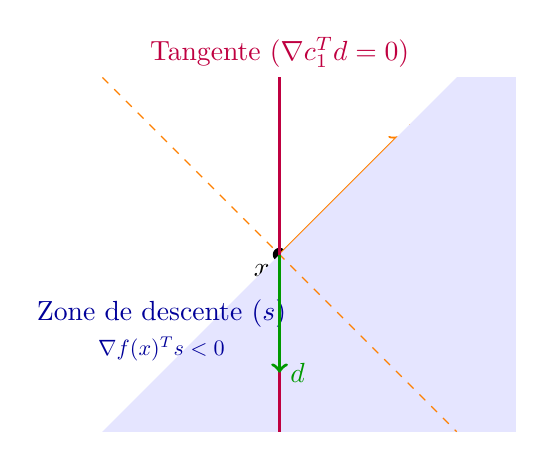
\begin{tikzpicture}[scale=1.5]
    % Point x
    \coordinate (x) at (0,0);
    \filldraw (x) circle (1.5pt) node[below left] {$x$};
    
    % Gradients
    \draw[->, orange, thick] (x) -- (1, 1) node[right] {$\nabla f(x)$};
    \draw[->, purple, thick] (x) -- (1, 0) node[right] {$\nabla c_1(x)$};
    
    % Descent zone (Blue zone) - Half plane defined by grad f . d < 0
    % Normal to grad f is (-1, 1). Line passing through origin.
    \begin{scope}
        \clip (-2, -1.5) rectangle (2, 1.5);
        % Fill region "opposite" to grad f
        % Rotate coordinate system so x-axis aligns with grad f? No, simpler.
        % Just fill a large rectangle rotated.
        \fill[blue!10, rotate=-135] (-3, 0) rectangle (3, 3);
    \end{scope}
    
    % Draw boundary of descent zone (orthogonal to grad f)
    \draw[dashed, orange] (-1.5, 1.5) -- (1.5, -1.5);
    \node[blue!60!black] at (-1, -0.5) {Zone de descente ($s$)};
    \node[blue!60!black, scale=0.8] at (-1, -0.8) {$\nabla f(x)^T s < 0$};
    
    % Tangent line (orthogonal to grad c1) -> Vertical line x=0
    \draw[thick, purple] (0, -1.5) -- (0, 1.5) node[above] {Tangente ($\nabla c_1^T d = 0$)};
    
    % In this specific drawing, the tangent line DOES intersect the blue zone (at the bottom)
    % grad f is at 45 deg, Blue zone is roughly 135 to 315 deg.
    % grad c1 is at 0 deg. Tangent is 90/-90 deg.
    % 90 deg is NOT in blue zone (prod with (1,1) is > 0)
    % -90 deg IS in blue zone (prod with (1,1) is < 0)
    % So there IS a descent direction here!
    
    \draw[->, green!60!black, very thick] (0, 0) -- (0, -1) node[right] {$d$};
    
\end{tikzpicture}
\caption{Illustration de la recherche de direction. La zone bleue représente l'ensemble des directions de descente (formant un angle obtus avec $\nabla f$). La droite verticale représente les directions tangentes à la contrainte. Ici, une direction $d$ existe (intersection de la droite et de la zone bleue), donc $x$ n'est pas un optimum.}
\label{fig:direction-finding}
\end{figure}

\begin{figureexplanation}
\textbf{Interprétation :} On cherche une direction $d$ telle que $\nabla f^T d < 0$ (descente) et $\nabla c_1^T d = 0$ (tangente). Si la droite tangente passe par la zone bleue, une telle direction existe et $x$ n'est pas optimal.
\end{figureexplanation}

\paragraph{Fonction Lagrangienne}
Définissons la fonction Lagrangienne :
\begin{equation}
    \mathcal{L}(x, \lambda_1) = f(x) - \lambda_1 c_1(x).
\end{equation}
Son gradient par rapport à $x$ est :
\begin{equation}
    \nabla_x \mathcal{L}(x, \lambda_1) = \nabla f(x) - \lambda_1 \nabla c_1(x).
\end{equation}
La condition de parallélisme des gradients peut alors être réécrite ainsi :
\begin{quote}
Il existe $\lambda_1^* \in \mathbb{R}$ tel que $\nabla_x \mathcal{L}(x^*, \lambda_1^*) = 0$.
\end{quote}
Cela suggère qu'il faut chercher les points stationnaires de $\mathcal{L}$ pour trouver les minimiseurs de $f$ sous contrainte.

\begin{remarque}
Le point $(1, 1)$ est également un point stationnaire de $\mathcal{L}$ (avec un multiplicateur de Lagrange différent). Il correspond ici au maximum global de $f$ sur le cercle.
\end{remarque}

\subsection{Une contrainte d'inégalité}

Considérons maintenant le problème avec une contrainte d'inégalité :
\begin{equation}
    \min_{(x_1, x_2) \in \mathbb{R}^2} x_1 + x_2 \quad \text{sous la contrainte} \quad 2 - x_1^2 - x_2^2 \geq 0.
\end{equation}
La contrainte est $c_1(x) = 2 - x_1^2 - x_2^2 \geq 0$. L'ensemble réalisable est le disque fermé de rayon $\sqrt{2}$. La solution est toujours le même point $x^* = (-1, -1)$.

Calculons les gradients en $x^*$ :
\begin{align*}
    \nabla f(x^*) &= \begin{pmatrix} 1 \\ 1 \end{pmatrix}, \\
    \nabla c_1(x) &= \begin{pmatrix} -2x_1 \\ -2x_2 \end{pmatrix} \implies \nabla c_1(x^*) = \begin{pmatrix} 2 \\ 2 \end{pmatrix}.
\end{align*}

La condition de parallélisme :
\begin{equation}
    \nabla f(x^*) = \lambda_1^* \nabla c_1(x^*)
\end{equation}
est satisfaite pour $\lambda_1^* = \frac{1}{2}$. Notez que cette fois, $\lambda_1^* > 0$.

\begin{remarque}[Interprétation du multiplicateur positif]
Le fait que $\lambda_1^* > 0$ indique que la contrainte est \textbf{bloquante} : relâcher cette contrainte permettrait de diminuer davantage $f$. En effet, si l'on pouvait "sortir" du disque (i.e.\ aller dans la direction $-\nabla f$), on pourrait continuer à diminuer la fonction objectif. Le multiplicateur $\lambda^*$ quantifie cette "pression" de la contrainte sur l'optimum.
\end{remarque}

\begin{figure}[H]
\centering
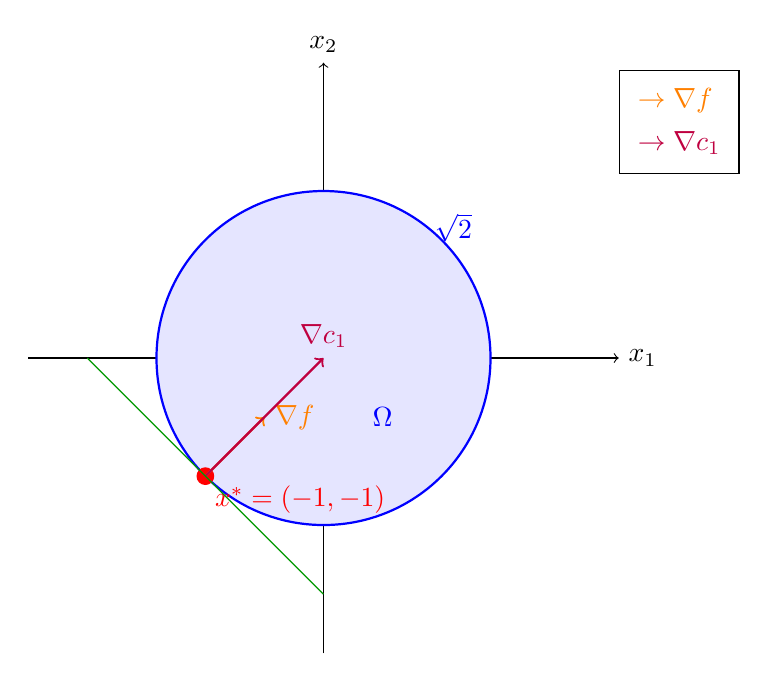
\begin{tikzpicture}[scale=1.5]
    % Axes
    \draw[->] (-2.5,0) -- (2.5,0) node[right] {$x_1$};
    \draw[->] (0,-2.5) -- (0,2.5) node[above] {$x_2$};
    
    % Feasible region (Disk)
    \filldraw[fill=blue!10, draw=blue, thick] (0,0) circle (1.414);
    \node[blue] at (0.5, -0.5) {$\Omega$};
    \node[blue] at (1.1, 1.1) {$\sqrt{2}$};
    
    % Optimal Point (-1, -1)
    \coordinate (Opt) at (-1,-1);
    \filldraw[red] (Opt) circle (2pt);
    \node[red, below right] at (-1, -1) {$x^* = (-1, -1)$};
    
    % Gradients at Opt
    % grad f is (1,1) -> visual (0.5, 0.5) points "inward" (towards origin)
    \draw[->, orange, thick] (Opt) -- ++(0.5, 0.5) node[right] {$\nabla f$};
    
    % grad c1 is (2,2) -> visual (1, 1) points "inward" (same direction)
    % Shifted slightly for visibility
    \draw[->, purple, thick] (Opt) -- ++(1.0, 1.0) node[above] {$\nabla c_1$};
    
    % Tangent line
    \draw[green!60!black, thin] (-2, 0) -- (0, -2);
    
    % Legend
    \matrix [draw, fill=white, right] at (2.5, 2) {
      \node[orange] {$\to \nabla f$}; \\
      \node[purple] {$\to \nabla c_1$}; \\
    };
\end{tikzpicture}
\caption{Minimisation avec contrainte d'inégalité. Au point optimal, $\nabla f$ et $\nabla c_1$ pointent dans la même direction ($\lambda^* > 0$).}
\label{fig:ex-inequality-constraint}
\end{figure}

\begin{figureexplanation}
\textbf{Interprétation :} Contrairement au cas d'égalité, les gradients pointent dans le \textbf{même sens}. Le multiplicateur $\lambda^* > 0$ traduit le fait que la contrainte "pousse" l'optimum : sans elle, on pourrait descendre davantage.
\end{figureexplanation}

\paragraph{Dérivation (Justification heuristique)}
Soit $x$ un point réalisable.
Un petit pas $s$ partant de $x$ produit une diminution de la fonction objectif si, au premier ordre :
\begin{equation}
    \nabla f(x)^T s < 0.
\end{equation}
Ce pas conserve la réalisabilité par rapport à la contrainte $c_1$ si :
\begin{equation}
    0 \le c_1(x+s) \approx c_1(x) + \nabla c_1(x)^T s.
\end{equation}
Ainsi, au premier ordre, on doit avoir :
\begin{equation}
    c_1(x) + \nabla c_1(x)^T s \ge 0.
\end{equation}

On distingue alors deux cas :
\begin{enumerate}
    \item \textbf{$x$ est strictement à l'intérieur du domaine} (i.e. $c_1(x) > 0$). \\
    Tout pas $s$ suffisamment petit garantira que $c_1(x) + \nabla c_1(x)^T s \ge 0$. Par exemple, on peut choisir la direction de la plus forte pente $s = -\alpha \nabla f(x)$ avec $\alpha > 0$ petit (si $\nabla f(x) \neq 0$). Dans ce cas, la contrainte n'est pas \textit{active} et ne limite pas localement la minimisation.
    
    \item \textbf{$x$ est sur la frontière de l'ensemble réalisable} (i.e. $c_1(x) = 0$). \\
    Dans ce cas, les conditions de diminution de la fonction et de réalisabilité deviennent :
    \begin{equation}
        \nabla f(x)^T s < 0 \quad \text{et} \quad \nabla c_1(x)^T s \ge 0.
    \end{equation}
    À l'optimum, il ne doit pas exister de tel $s$. Cela implique une relation spécifique entre les gradients (voir condition KKT plus loin).
\end{enumerate}



\begin{figure}[H]
\centering
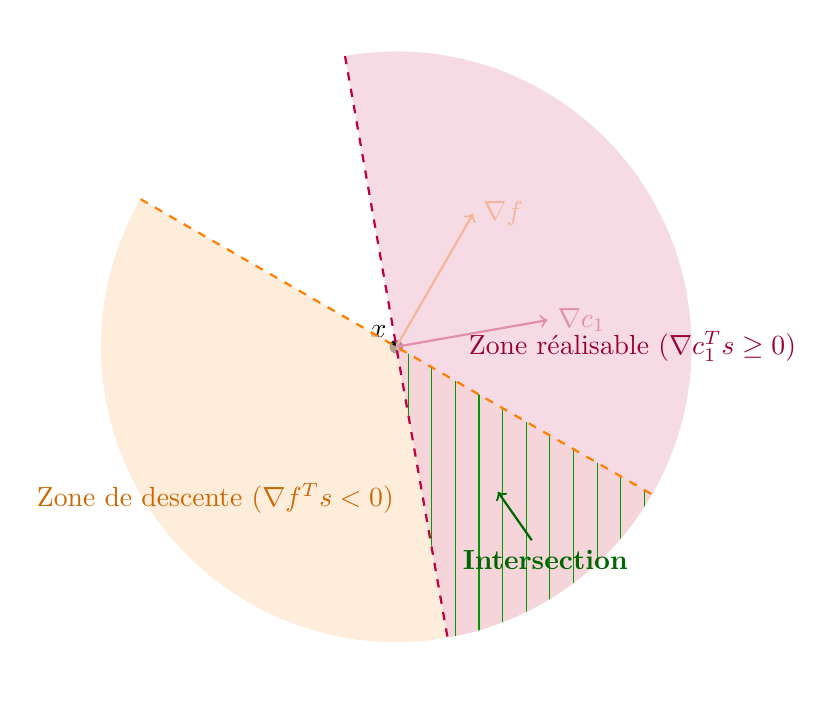
\begin{tikzpicture}[scale=1.5]
    % Point x
    \coordinate (x) at (0,0);
    \filldraw (x) circle (1.5pt) node[above left] {$x$};
    
    % Vectors setup
    % grad f at 60 degrees
    \draw[->, orange, thick] (x) -- (60:1.3) node[right] {$\nabla f$};
    % grad c1 moved to 10 degrees (closer to grad f to tighten intersection)
    \draw[->, purple, thick] (x) -- (10:1.3) node[right] {$\nabla c_1$};
    
    % Half-Plane 1: Descent (Orange)
    % Perpendicular to grad f (150 to 330).
    \begin{scope}
        \fill[orange!20, opacity=0.7] (0,0) -- (150:2.5) arc (150:330:2.5) -- cycle;
    \end{scope}
     \node[orange!80!black] at (220:2.0) {Zone de descente ($\nabla f^T s < 0$)};

    % Half-Plane 2: Feasible (Purple)
    % Perpendicular to grad c1 (normal at 10 deg -> boundary at 100/280).
    % Valid region is same side as grad c1 -> Angles [-80, 100] i.e. [280, 460].
    \begin{scope}
        \fill[purple!20, opacity=0.7] (0,0) -- (100:2.5) arc (100:-80:2.5) -- cycle;
    \end{scope}
    \node[purple!80!black] at (0:2.0) {Zone réalisable ($\nabla c_1^T s \geq 0$)};

    % Intersection (Green hatching)
    % Intersection of [150, 330] and [280, 460] is [280, 330].
    % Width = 50 degrees (tighter than 90).
    \begin{scope}
        \clip (0,0) -- (280:2.5) arc (280:330:2.5) -- cycle;
        \foreach \x in {-2.5,-2.3,...,2.5} \draw[green!60!black, thin] (\x,-2.5) -- (\x,2.5);
    \end{scope}
    
    % Boundaries lines
    \draw[dashed, orange, thick] (150:2.5) -- (330:2.5);
    \draw[dashed, purple, thick] (100:2.5) -- (280:2.5); % Boundary for grad c1 at 10 deg

    % Label Acceptable Directions
    \node[green!40!black, font=\bfseries] at (305:2.2) {Intersection};
    \draw[->, green!40!black, thick] (305:2.0) -- (305:1.5);
    
\end{tikzpicture}
\caption{Visualisation des directions admissibles. Les deux zones colorées (orange pour la descente, violet pour la réalisabilité) se chevauchent. L'intersection (hachurée en vert) représente l'ensemble des directions admissibles.}
\label{fig:acceptable-directions-overlap}
\end{figure}

\begin{figureexplanation}
\textbf{Interprétation géométrique :}
\begin{itemize}
    \item Pour qu'une direction $s$ soit \textbf{de descente}, elle doit faire un angle obtus avec le gradient de la fonction objectif $\nabla f$ (zone orange).
    \item Pour qu'elle soit \textbf{réalisable} (au premier ordre), elle doit pointer vers l'intérieur du domaine par rapport à la contrainte active, donc faire un angle aigu avec le gradient de la contrainte $\nabla c_1$ (zone violette).
    \item L'\textbf{intersection} (hachures vertes) contient les directions admissibles. Tant que cette intersection n'est pas vide, on peut améliorer la solution.
\end{itemize}
\end{figureexplanation}

La question fondamentale devient alors : \textbf{Quand n'y a-t-il aucune direction admissible ?}

\begin{figure}[H]
\centering
\begin{subfigure}[b]{0.45\textwidth}
    \centering
    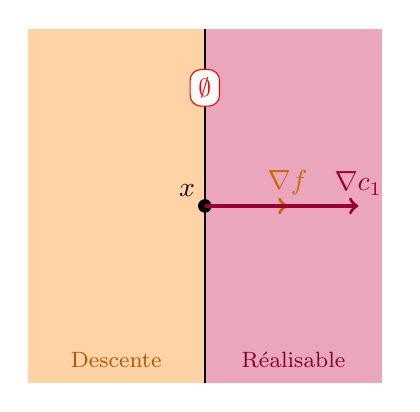
\begin{tikzpicture}[scale=1.5]
        % CASE 1: No acceptable direction - CLEAN VERSION
        \coordinate (x) at (0,0);
        
        % Zone de descente (left, orange transparent)
        \fill[orange, opacity=0.35] (-1.5,-1.5) rectangle (0,1.5);
        
        % Zone réalisable (right, purple transparent)
        \fill[purple, opacity=0.35] (0,-1.5) rectangle (1.5,1.5);
        
        % Boundary line
        \draw[thick, black] (0,-1.5) -- (0,1.5);
        
        % Point
        \filldraw (x) circle (1.5pt) node[above left] {$x$};
        
        % Gradients (parallel, same direction)
        \draw[->, orange!80!black, very thick] (x) -- (0.7, 0) node[above] {$\nabla f$};
        \draw[->, purple!80!black, very thick] (x) -- (1.3, 0) node[above] {$\nabla c_1$};
        
        % Labels at bottom, well separated
        \node[orange!70!black, font=\footnotesize] at (-0.75, -1.3) {Descente};
        \node[purple!70!black, font=\footnotesize] at (0.75, -1.3) {Réalisable};
        
        % "Intersection vide" label
        \node[red, font=\small\bfseries, fill=white, draw=red, inner sep=3pt, rounded corners] at (0, 1.0) {$\emptyset$};
        
    \end{tikzpicture}
    \caption{Gradients alignés : zones disjointes, aucune direction admissible.}
\end{subfigure}
\hfill
\begin{subfigure}[b]{0.45\textwidth}
    \centering
    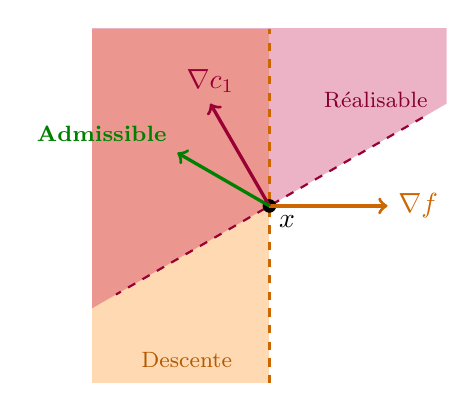
\begin{tikzpicture}[scale=1.5]
        % CASE 2: Overlapping transparent zones
        \coordinate (x) at (0,0);
        
        \begin{scope}
            \clip (-1.5,-1.5) rectangle (1.5,1.5);
            
            % Zone de descente (orange, transparent)
            \fill[orange, opacity=0.3] (-1.5,-1.5) rectangle (0,1.5);
            
            % Zone réalisable (purple, transparent) - overlaps naturally
            \fill[purple, opacity=0.3] (0,0) -- (30:3) arc (30:210:3) -- cycle;
        \end{scope}
        
        % Boundaries
        \draw[dashed, orange!80!black, thick] (0, -1.5) -- (0, 1.5);
        \draw[dashed, purple!80!black, thick] (30:1.5) -- (210:1.5);
        
        % Point
        \filldraw (x) circle (1.5pt) node[below right] {$x$};
        
        % Gradients
        \draw[->, orange!80!black, very thick] (x) -- (1, 0) node[right] {$\nabla f$};
        \draw[->, purple!80!black, very thick] (x) -- (120:1.0) node[above] {$\nabla c_1$};
        
        % Labels positioned OUTSIDE overlap
        \node[orange!70!black, font=\footnotesize] at (-0.7, -1.3) {Descente};
        \node[purple!70!black, font=\footnotesize] at (0.9, 0.9) {Réalisable};
        
        % Arrow indicating intersection zone
        \draw[->, green!50!black, very thick] (x) -- (150:0.9) node[above left, font=\footnotesize\bfseries] {Admissible};
        
    \end{tikzpicture}
    \caption{Cas régulier : L'intersection des zones (mélange des couleurs) donne les directions admissibles.}
\end{subfigure}
\caption{Comparaison des configurations "Demi-plans". À gauche, les gradients parallèles de même sens créent une obstruction totale (opposition parfaite des zones).}
\label{fig:admissible-comparison}
\end{figure}

\begin{figureexplanation}
\textbf{Interprétation géométrique :}
\begin{itemize}
    \item \textbf{Cas (a) :} Les zones de descente et de réalisabilité sont disjointes (aucun chevauchement). C'est la condition d'optimalité.
    \item \textbf{Cas (b) :} Les deux zones se chevauchent via la transparence des couleurs. L'intersection (plus foncée) donne les directions admissibles.
\end{itemize}
\end{figureexplanation}

On en déduit la conclusion suivante :
\begin{quote}
Il n'existe aucune direction admissible lorsque les gradients sont parallèles et pointent dans la même direction :
\begin{equation}
    \nabla f(x) = \lambda \nabla c_1(x) \quad \text{avec } \lambda > 0.
\end{equation}
\end{quote}

\paragraph{Résumé sur les deux cas (Conditions d'optimalité)}
Lorsqu'il n'existe aucune direction de descente réalisable, on a le système suivant :
\begin{equation}
    \begin{cases}
        \nabla_x \mathcal{L}(x, \lambda_1^*) = 0 \quad \text{pour un certain } \lambda_1^* \ge 0, \\
        \lambda_1^* c_1(x) = 0.
    \end{cases}
\end{equation}
La seconde équation est appelée \textbf{condition de complémentarité} ("Complementarity condition").
Elle signifie que le multiplicateur $\lambda_1^*$ ne peut être (strictement) positif que si la contrainte $c_1$ est active ($c_1(x)=0$).

Rappelons la définition du Lagrangien :
\begin{equation}
    \mathcal{L}(x, \lambda_1) = f(x) - \lambda_1 c_1(x).
\end{equation}
Si $\lambda_1 = 0$, alors $\mathcal{L}(x, \lambda_1) = f(x)$ et $\nabla_x \mathcal{L} = \nabla f(x)$. Cela correspond au cas où l'optimum se trouve à l'intérieur du domaine (contrainte inactive), et la condition classique $\nabla f(x) = 0$ est retrouvée.

\subsection{Deux contraintes d'inégalité}

Considérons le problème suivant :
\begin{equation}
    \min_{(x_1, x_2) \in \mathbb{R}^2} x_1 + x_2 \quad \text{sous les contraintes} \quad 
    \begin{cases}
        2 - x_1^2 - x_2^2 \ge 0, \\
        x_2 \ge 0.
    \end{cases}
\end{equation}
L'ensemble réalisable est la moitié supérieure du disque de rayon $\sqrt{2}$.
Le point optimal est $x^* = (-\sqrt{2}, 0)$.

Calculons les gradients en ce point :
\begin{align*}
    \nabla f(x) &= \begin{pmatrix} 1 \\ 1 \end{pmatrix}, \\
    \nabla c_1(x) &= \begin{pmatrix} -2x_1 \\ -2x_2 \end{pmatrix} \implies \nabla c_1(x^*) = \begin{pmatrix} 2\sqrt{2} \\ 0 \end{pmatrix}, \\
    \nabla c_2(x) &= \begin{pmatrix} 0 \\ 1 \end{pmatrix} \implies \nabla c_2(x^*) = \begin{pmatrix} 0 \\ 1 \end{pmatrix}.
\end{align*}
Remarquons que les deux contraintes sont actives en $x^*$ ($c_1(x^*) = 0$ et $c_2(x^*) = 0$).

On s'attendrait à ce qu'une direction de descente réalisable $d$ satisfasse :
\begin{equation}
    \begin{cases}
        \nabla c_i(x^*)^T d \ge 0 \quad \text{pour } i=1, 2 \quad \text{(réalisable)}, \\
        \nabla f(x^*)^T d < 0 \quad \text{(descente)}.
    \end{cases}
\end{equation}

\begin{figure}[H]
\centering
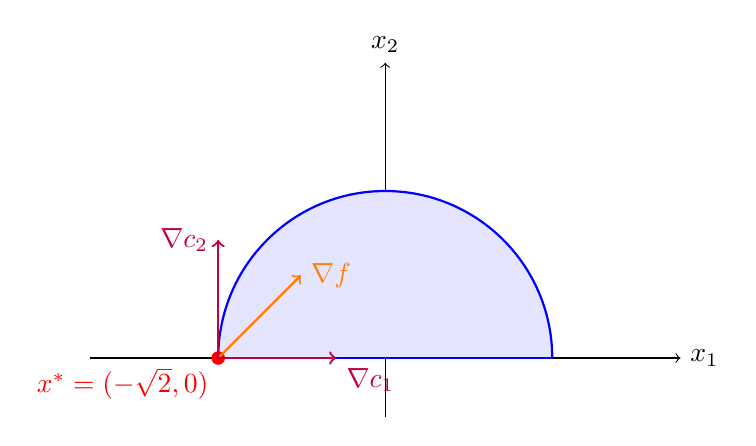
\begin{tikzpicture}[scale=1.5]
    % Axes
    \draw[->] (-2.5,0) -- (2.5,0) node[right] {$x_1$};
    \draw[->] (0,-0.5) -- (0,2.5) node[above] {$x_2$};
    
    % Feasible region: Upper semi-disk
    \fill[blue!10] (1.414, 0) arc (0:180:1.414) -- cycle;
    \draw[blue, thick] (1.414, 0) arc (0:180:1.414);
    \draw[blue, thick] (-1.414, 0) -- (1.414, 0);
    
    % Optimal point
    \coordinate (Opt) at (-1.414, 0);
    \filldraw[red] (Opt) circle (1.5pt) node[below left] {$x^* = (-\sqrt{2}, 0)$};
    
    % Gradients at Opt
    % grad f = (1, 1). Visual scaled 0.7
    \draw[->, orange, thick] (Opt) -- ++(0.7, 0.7) node[right] {$\nabla f$};
    
    % grad c1 = (2sqrt(2), 0) approx (2.8, 0). Points Right. Visual scaled 1.0
    \draw[->, purple, thick] (Opt) -- ++(1.0, 0) node[below right] {$\nabla c_1$};
    
    % grad c2 = (0, 1). Points Up. Visual scaled 1.0
    \draw[->, purple, thick] (Opt) -- ++(0, 1.0) node[left] {$\nabla c_2$};
    
    % Cone of feasible directions?
    % Feasible directions roughly Right-Up sector
    % Descent directions roughly Left-Down sector
    % No interaction.
    
\end{tikzpicture}
\caption{Exemple avec deux contraintes actives. Les deux contraintes (disque et positivité) sont actives en $x^*$.}
\label{fig:ex-two-inequalities}
\end{figure}

\begin{figureexplanation}
\textbf{Situation avec plusieurs contraintes actives :}
Ici, le point $x^*$ est à l'intersection de deux frontières ($c_1=0$ pour le cercle, $c_2=0$ pour la droite horizontale).
\begin{itemize}
    \item Le gradient $\nabla f$ doit être une combinaison linéaire à coefficients positifs des gradients des contraintes actives ($\nabla c_1$ et $\nabla c_2$).
    \item Géométriquement, cela signifie que $-\nabla f$ (direction de descente souhaitée) pointe à l'extérieur du cône formé par les tangentes aux contraintes. On est "bloqué" par les deux murs à la fois.
\end{itemize}
\end{figureexplanation}

\paragraph{Modification du Lagrangien}
Pour ce problème à deux contraintes, on définit le Lagrangien :
\begin{equation}
    \mathcal{L}(x, \lambda) = f(x) - \lambda_1 c_1(x) - \lambda_2 c_2(x).
\end{equation}
Les conditions deviennent :
\begin{itemize}
    \item $\nabla_x \mathcal{L}(x^*, \lambda^*) = 0$ avec $\lambda^* \ge 0$ (i.e., $\lambda_1^* \ge 0$ et $\lambda_2^* \ge 0$).
    \item Conditions de complémentarité : $\lambda_1^* c_1(x^*) = 0$ et $\lambda_2^* c_2(x^*) = 0$.
\end{itemize}

Vérifions ces conditions pour notre point $x^* = (-\sqrt{2}, 0)$.
On cherche $\lambda_1^*, \lambda_2^*$ tels que :
\begin{align*}
    \nabla f(x^*) - \lambda_1^* \nabla c_1(x^*) - \lambda_2^* \nabla c_2(x^*) &= 0 \\
    \begin{pmatrix} 1 \\ 1 \end{pmatrix} - \lambda_1^* \begin{pmatrix} 2\sqrt{2} \\ 0 \end{pmatrix} - \lambda_2^* \begin{pmatrix} 0 \\ 1 \end{pmatrix} &= \begin{pmatrix} 0 \\ 0 \end{pmatrix}.
\end{align*}
Ce système donne :
\begin{equation}
    \begin{cases}
        1 - 2\sqrt{2} \lambda_1^* = 0 \implies \lambda_1^* = \frac{1}{2\sqrt{2}} > 0, \\
        1 - \lambda_2^* = 0 \implies \lambda_2^* = 1 > 0.
    \end{cases}
\end{equation}
Les multiplicateurs sont positifs, ce qui est cohérent avec le fait que les deux contraintes sont actives et limitent la descente.
\paragraph{Analyse d'un autre point candidat}
Considérons le point $x = (\sqrt{2}, 0)$. Ce point est réalisable (sur la frontière).
Vérifions si les conditions d'optimalité sont satisfaites.
\begin{align*}
    \nabla f(x) &= \begin{pmatrix} 1 \\ 1 \end{pmatrix}, \\
    \nabla c_1(x) &= \begin{pmatrix} -2\sqrt{2} \\ 0 \end{pmatrix}, \\
    \nabla c_2(x) &= \begin{pmatrix} 0 \\ 1 \end{pmatrix}.
\end{align*}
On cherche $\lambda_1^*, \lambda_2^*$ tels que :
\begin{equation}
    \begin{pmatrix} 1 \\ 1 \end{pmatrix} - \lambda_1^* \begin{pmatrix} -2\sqrt{2} \\ 0 \end{pmatrix} - \lambda_2^* \begin{pmatrix} 0 \\ 1 \end{pmatrix} = \begin{pmatrix} 0 \\ 0 \end{pmatrix}.
\end{equation}
Cela donne le système :
\begin{equation}
    \begin{cases}
        1 + 2\sqrt{2} \lambda_1^* = 0 \implies \lambda_1^* = -\frac{1}{2\sqrt{2}} < 0, \\
        1 - \lambda_2^* = 0 \implies \lambda_2^* = 1 \ge 0.
    \end{cases}
\end{equation}
Ici, on trouve $\lambda_1^* < 0$. La condition KKT $\lambda^* \ge 0$ n'est pas respectée.
\textbf{Conclusion :} Le point $x = (\sqrt{2}, 0)$ n'est pas un minimum local (en effet, on pourrait augmenter $x_1$ pour diminuer $f$ tout en restant dans le domaine).

\section{Cône tangent et qualifications des contraintes}

Dans cette section, nous étudierons les conditions sous lesquelles les points de vue analytique et géométrique coïncident ("conditions under which analytical and geometrical points of view coincide").

\subsection{Définitions}

\begin{definition}[Suite réalisable]
    Une suite $(z_k)_k$ est dite \textbf{suite réalisable approximant le point réalisable} $x$ si :
    \begin{itemize}
        \item $z_k \to x$ quand $k \to \infty$,
        \item $z_k \in \Omega$ pour $k$ assez grand.
    \end{itemize}
\end{definition}

\begin{definition}[Vecteur tangent]
    Un vecteur $d \in \mathbb{R}^n$ est dit \textbf{tangent} (ou vecteur tangent) à $\Omega$ au point réalisable $x$ s'il existe une suite réalisable $(z_k)_k$ approximant $x$ et une suite de scalaires positifs $(t_k)_k$ avec $t_k \to 0$ tels que :
    \begin{equation}
        \lim_{k \to \infty} \frac{z_k - x}{t_k} = d.
    \end{equation}
\end{definition}



L'ensemble des vecteurs tangents à $\Omega$ en $x$ est noté $T_\Omega(x)$ et est appelé \textbf{cône tangent} à $\Omega$ en $x$.

\begin{remarque}
    $T_\Omega(x)$ est bien un cône :
    \begin{itemize}
        \item $0 \in T_\Omega(x)$ (prendre la suite constante $z_k = x$).
        \item Si $d \in T_\Omega(x)$, alors pour tout $\alpha > 0$, $\alpha d \in T_\Omega(x)$. \\
        En effet, il suffit de remplacer la suite $(t_k)_k$ par $(t'_k)_k$ définie par $t'_k = \alpha^{-1} t_k$. Comme $t_k \to 0$, on a aussi $t'_k \to 0$, et
        \[ \lim_{k \to \infty} \frac{z_k - x}{t'_k} = \lim_{k \to \infty} \alpha \frac{z_k - x}{t_k} = \alpha d. \]
    \end{itemize}
\end{remarque}

\begin{definition}[Conditions réalisables linéarisées]
    Étant donné un point réalisable $x$ et l'ensemble des contraintes actives $\mathcal{A}(x)$, l'ensemble des \textbf{directions réalisables linéarisées} $\mathcal{F}(x)$ est défini par :
    \begin{equation}
        \mathcal{F}(x) = \left\{ d \in \mathbb{R}^n \mid 
        \begin{aligned}
            d^T \nabla c_i(x) &= 0 \quad \forall i \in \mathcal{E}, \\
            d^T \nabla c_i(x) &\ge 0 \quad \forall i \in \mathcal{I} \cap \mathcal{A}(x)
        \end{aligned}
        \right\}.
    \end{equation}
\end{definition}

\begin{remarque}
    $\mathcal{F}(x)$ est aussi un cône.
\end{remarque}

\begin{exemple}[Cône tangent pour une contrainte d'égalité]
    Considérons le problème :
    \begin{equation}
        \min_{x \in \mathbb{R}^2} x_1 + x_2 \quad \text{sous la contrainte} \quad x_1^2 + x_2^2 - 2 = 0.
    \end{equation}
    Soit $x = (-\sqrt{2}, 0)$.
    Les \textbf{suites réalisables} $(z_k)_k$ approchant $x$ doivent se trouver sur le cercle.
    
    Considérons les suites réalisables :
    \begin{equation}
        z_k = \left(-\sqrt{2 - \frac{1}{k^2}}, \frac{1}{k}\right) \quad \text{ou} \quad z'_k = \left(-\sqrt{2 - \frac{1}{k^2}}, -\frac{1}{k}\right).
    \end{equation}
    Vérifions qu'elles sont sur le cercle : $\left(-\sqrt{2-1/k^2}\right)^2 + (\pm 1/k)^2 = 2 - 1/k^2 + 1/k^2 = 2$.
    
    Avec $t_k = \|z_k - x\|$, on trouve que les vecteurs $(0, 1)$ et $(0, -1)$ sont tangents.
    Plus généralement, l'ensemble des vecteurs tangents est la droite verticale :
    \begin{equation}
        T_\Omega(x) = \{ (0, d_2) \mid d_2 \in \mathbb{R} \}.
    \end{equation}

    \begin{center}
    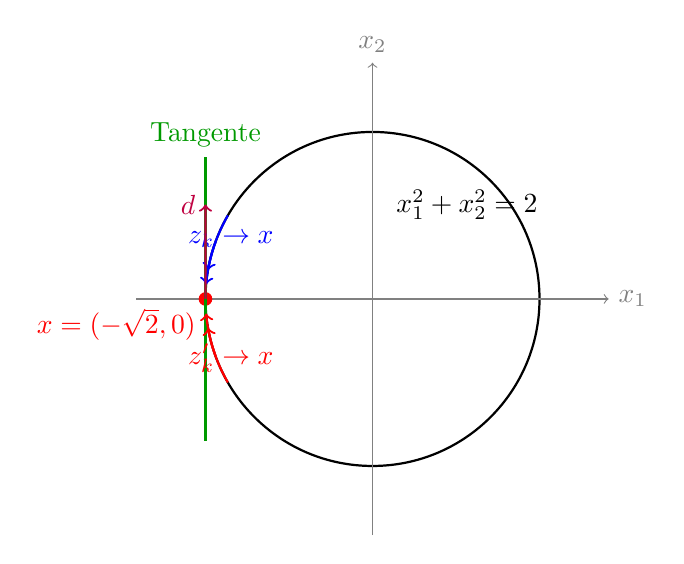
\begin{tikzpicture}[scale=1.5]
        % Circle
        \draw[thick] (0,0) circle (1.414);
        \node at (0.8, 0.8) {$x_1^2+x_2^2=2$};
        
        % Axes
        \draw[->, gray] (-2,0) -- (2,0) node[right] {$x_1$};
        \draw[->, gray] (0,-2) -- (0,2) node[above] {$x_2$};
        
        % Point x
        \coordinate (x) at (-1.414, 0);
        \filldraw[red] (x) circle (1.5pt) node[below left] {$x = (-\sqrt{2}, 0)$};
        
        % Tangent line (vertical)
        \draw[green!60!black, thick] (-1.414, -1.2) -- (-1.414, 1.2) node[above] {Tangente};
        
        % Converging arrows (Feasible sequences) (Red and Blue)
        % From top (z_k): Blue arrows approaching 180 deg from 150 deg
        \draw[->, blue, thick] (150:1.414) arc (150:170:1.414);
        \draw[->, blue, thick] (160:1.414) arc (160:175:1.414);
        \node[blue] at (-1.2, 0.5) {$z_k \to x$};

        % From bottom (z'_k): Red arrows approaching 180 deg from 210 deg
        \draw[->, red, thick] (210:1.414) arc (210:190:1.414);
        \draw[->, red, thick] (200:1.414) arc (200:185:1.414);
        \node[red] at (-1.2, -0.5) {$z'_k \to x$};
        
        % Vector d (tangent vector)
        \draw[->, purple, thick] (x) -- (-1.414, 0.8) node[left] {$d$};

    \end{tikzpicture}
    \end{center}
\end{exemple}

Calculons maintenant $\mathcal{F}(x)$ en $x = (-\sqrt{2}, 0)$.
    On a $\mathcal{E} = \{1\}$ et $\mathcal{I} = \emptyset$, donc $\mathcal{A}(x) = \{1\}$. 
    La contrainte $c_1(x) = x_1^2 + x_2^2 - 2$ a pour gradient :
    \begin{equation}
        \nabla c_1(x) = \begin{pmatrix} 2x_1 \\ 2x_2 \end{pmatrix} \implies \nabla c_1(x) = \begin{pmatrix} -2\sqrt{2} \\ 0 \end{pmatrix}.
    \end{equation}
    L'ensemble des directions réalisables linéarisées est :
    \begin{equation}
        \mathcal{F}(x) = \left\{ d = \begin{pmatrix} d_1 \\ d_2 \end{pmatrix} \in \mathbb{R}^2 \mid d^T \nabla c_1(x) = 0 \right\}.
    \end{equation}
    La condition $d^T \nabla c_1(x) = 0$ donne :
    \begin{equation}
        \begin{pmatrix} d_1 \\ d_2 \end{pmatrix}^T \begin{pmatrix} -2\sqrt{2} \\ 0 \end{pmatrix} = -2\sqrt{2} d_1 = 0 \implies d_1 = 0.
    \end{equation}
    Donc :
    \begin{equation}
        \mathcal{F}(x) = \left\{ (0, d_2)^T \mid d_2 \in \mathbb{R} \right\} = T_\Omega(x).
    \end{equation}

\begin{remarque}[Cas où $\mathcal{F}(x) \neq T_\Omega(x)$]
    \begin{itemize}
        \item Si on change la contrainte pour $(x_1^2 + x_2^2 - 2)^2 = 0$, on peut montrer que $\mathcal{F}(x) = \mathbb{R}^2 \neq T_\Omega(x)$.
        
        En effet, le gradient de cette nouvelle contrainte en $x$ s'annule :
        \[ \nabla \left[ (x_1^2 + x_2^2 - 2)^2 \right] = 2(x_1^2 + x_2^2 - 2) \cdot \begin{pmatrix} 2x_1 \\ 2x_2 \end{pmatrix} = 0 \text{ sur le cercle.} \]
        Donc la condition $d^T \nabla c(x) = 0$ est toujours satisfaite, d'où $\mathcal{F}(x) = \mathbb{R}^2$.
        
        \item Si on change la contrainte pour $2 - x_1^2 - x_2^2 \geq 0$ (inégalité), alors :
        \begin{equation}
            T_\Omega(x) = \left\{ (d_1, d_2)^T \in \mathbb{R}^2 \mid d_1 \geq 0 \right\} = \mathcal{F}(x).
        \end{equation}
    \end{itemize}
\end{remarque}

\subsection{Qualification des contraintes (LICQ)}

\begin{definition}[LICQ -- Linear Independence Constraint Qualification]
    Étant donné un point réalisable $x \in \Omega$ et l'ensemble actif $\mathcal{A}(x)$, on dit que la condition \textbf{LICQ} (\\textit{Linear Independence Constraint Qualification}) est satisfaite en $x$ si l'ensemble des gradients des contraintes actives
    \begin{equation}
        \left\{ \nabla c_i(x) \mid i \in \mathcal{A}(x) \right\}
    \end{equation}
    est \textbf{linéairement indépendant}.
\end{definition}

\begin{proposition}
    Sous la condition LICQ, le cône tangent $T_\Omega(x)$ et l'ensemble des directions réalisables linéarisées $\mathcal{F}(x)$ coïncident :
    \begin{equation}
        T_\Omega(x) = \mathcal{F}(x).
    \end{equation}
\end{proposition}

\begin{lemme}[Cas des contraintes linéaires]
    Supposons qu'en un point $x^* \in \Omega$, toutes les contraintes actives $c_i$ (pour $i \in \mathcal{A}(x^*)$) soient des fonctions \textbf{linéaires} (ou affines). Alors :
    \begin{equation}
        T_\Omega(x^*) = \mathcal{F}(x^*).
    \end{equation}
\end{lemme}

\begin{remarque}
    Ce lemme est un cas particulier de la proposition précédente. Les contraintes linéaires satisfont automatiquement LICQ si leurs gradients sont linéairement indépendants. De plus, pour les contraintes affines, l'approximation linéaire est exacte, ce qui explique l'égalité $T_\Omega = \mathcal{F}$.
\end{remarque}

\section{Conditions d'optimalité}

Dans cette section, nous formalisons les conditions d'optimalité pour les problèmes d'optimisation sous contraintes. Pour les preuves détaillées, nous renvoyons à Nocedal et Wright \cite{nocedal2006numerical}.

\subsection{La fonction Lagrangienne}

\begin{definition}[Fonction Lagrangienne]
    Pour le problème d'optimisation
    \begin{equation}
        \min_{x \in \mathbb{R}^n} f(x) \quad \text{sous les contraintes} \quad c_i(x) \begin{cases} = 0 & \text{si } i \in \mathcal{E}, \\ \geq 0 & \text{si } i \in \mathcal{I}, \end{cases}
    \end{equation}
    la \textbf{fonction Lagrangienne} est définie par :
    \begin{equation}
        \mathcal{L}(x, \lambda) = f(x) - \sum_{i \in \mathcal{E} \cup \mathcal{I}} \lambda_i c_i(x),
    \end{equation}
    où $\lambda = (\lambda_i)_{i \in \mathcal{E} \cup \mathcal{I}}$ est le vecteur des \textbf{multiplicateurs de Lagrange}.
\end{definition}

\begin{remarque}
    La convention de signe peut varier selon les auteurs. Notre choix (signe moins devant les $\lambda_i$) implique que pour les contraintes d'inégalité, les multiplicateurs optimaux seront positifs $\lambda_i^* \geq 0$, ce qui correspond à l'interprétation économique standard.
\end{remarque}

\subsection{Conditions KKT}

\begin{theoreme}[Conditions de Karush-Kuhn-Tucker (KKT)]
    Soit $x^*$ un minimum local du problème d'optimisation. Si LICQ est satisfaite en $x^*$, alors il existe un vecteur de multiplicateurs $\lambda^* = (\lambda_i^*)_{i \in \mathcal{E} \cup \mathcal{I}}$ tel que :
    \begin{enumerate}
        \item \textbf{Stationnarité :} 
        \begin{equation}
            \nabla_x \mathcal{L}(x^*, \lambda^*) = \nabla f(x^*) - \sum_{i \in \mathcal{E} \cup \mathcal{I}} \lambda_i^* \nabla c_i(x^*) = 0.
        \end{equation}
        
        \item \textbf{Réalisabilité primale :}
        \begin{equation}
            c_i(x^*) = 0 \quad \forall i \in \mathcal{E}, \qquad c_i(x^*) \geq 0 \quad \forall i \in \mathcal{I}.
        \end{equation}
        
        \item \textbf{Réalisabilité duale :}
        \begin{equation}
            \lambda_i^* \geq 0 \quad \forall i \in \mathcal{I}.
        \end{equation}
        (Pas de contrainte de signe pour $\lambda_i^*$ avec $i \in \mathcal{E}$.)
        
        \item \textbf{Complémentarité :}
        \begin{equation}
            \lambda_i^* c_i(x^*) = 0 \quad \forall i \in \mathcal{I}.
        \end{equation}
    \end{enumerate}
\end{theoreme}

\begin{remarque}[Interprétation de la complémentarité]
    La condition de complémentarité $\lambda_i^* c_i(x^*) = 0$ signifie que :
    \begin{itemize}
        \item Si une contrainte d'inégalité $i \in \mathcal{I}$ n'est pas active ($c_i(x^*) > 0$), alors le multiplicateur correspondant doit être nul ($\lambda_i^* = 0$).
        \item Un multiplicateur strictement positif ($\lambda_i^* > 0$) ne peut apparaître que si la contrainte est active ($c_i(x^*) = 0$).
    \end{itemize}
    Intuitivement, seules les contraintes ``serrées'' exercent une ``force'' sur l'optimum.
\end{remarque}

\subsection{Conditions du second ordre}

\paragraph{Hypothèse.} Dans cette section III.2, nous supposons que $f$ et les $c_i$ sont \textbf{deux fois continûment différentiables}.

\begin{definition}[Cône critique]
    Étant donné $\mathcal{A}(x^*)$ et des multiplicateurs de Lagrange $\lambda^*$ satisfaisant les conditions KKT, le \textbf{cône critique} $\mathcal{C}(x^*, \lambda^*)$ est défini par :
    \begin{equation}
        \mathcal{C}(x^*, \lambda^*) = \left\{ w \in \mathcal{F}(x^*) \mid \nabla c_i(x^*)^T w = 0 \ \text{pour tout } i \in \mathcal{I} \cap \mathcal{A}(x^*) \ \text{avec } \lambda_i^* > 0 \right\}.
    \end{equation}
\end{definition}

\begin{remarque}
    Le cône critique est un sous-ensemble de l'ensemble des directions réalisables linéarisées $\mathcal{F}(x^*)$. Il contient les directions ``critiques'' qui sont orthogonales aux gradients des contraintes d'inégalité qui sont à la fois actives \textbf{et} qui ont un multiplicateur strictement positif.
    
    Intuitivement, ce sont les directions le long desquelles la contrainte ``compte vraiment'' car elle exerce une force non nulle sur l'optimum.
\end{remarque}

\begin{remarque}[Équivalence pour le cône critique]
    De manière équivalente, on peut caractériser le cône critique par :
    \begin{equation}
        w \in \mathcal{C}(x^*, \lambda^*) \iff 
        \begin{cases}
            \nabla c_i(x^*)^T w = 0 & \text{pour tout } i \in \mathcal{E}, \\
            \nabla c_i(x^*)^T w \geq 0 & \text{pour tout } i \in \mathcal{I} \cap \mathcal{A}(x^*) \text{ avec } \lambda_i^* = 0, \\
            \nabla c_i(x^*)^T w = 0 & \text{pour tout } i \in \mathcal{I} \cap \mathcal{A}(x^*) \text{ avec } \lambda_i^* > 0.
        \end{cases}
    \end{equation}
    Autrement dit, les directions du cône critique ``adhèrent'' aux contraintes d'égalité et aux contraintes d'inégalité actives lorsqu'on perturbe légèrement la fonction objectif.
    
    \paragraph{Propriété fondamentale.}
    On a la propriété importante suivante :
    \begin{equation}
        w \in \mathcal{C}(x^*, \lambda^*) \implies \lambda_i^* \nabla c_i(x^*)^T w = 0 \quad \forall i \in \mathcal{E} \cup \mathcal{I}.
    \end{equation}
    En effet :
    \begin{itemize}
        \item Pour $i \in \mathcal{E}$, on a $\nabla c_i(x^*)^T w = 0$ par définition de $\mathcal{F}(x^*)$.
        \item Pour $i \in \mathcal{I} \cap \mathcal{A}(x^*)$ avec $\lambda_i^* > 0$, on a $\nabla c_i(x^*)^T w = 0$ par définition de $\mathcal{C}(x^*, \lambda^*)$.
        \item Pour $i \in \mathcal{I} \cap \mathcal{A}(x^*)$ avec $\lambda_i^* = 0$, le produit $\lambda_i^* \nabla c_i(x^*)^T w = 0$.
        \item Pour $i \in \mathcal{I} \setminus \mathcal{A}(x^*)$ (contraintes inactives), on a $\lambda_i^* = 0$ par complémentarité.
    \end{itemize}
    
    \paragraph{Conséquence.} Puisque $\nabla_x \mathcal{L}(x^*, \lambda^*) = 0$ par la condition KKT de stationnarité, on a :
    \begin{equation}
        w \in \mathcal{C}(x^*, \lambda^*) \implies w^T \nabla f(x^*) = w^T \sum_{i \in \mathcal{E} \cup \mathcal{I}} \lambda_i^* \nabla c_i(x^*) = \sum_{i \in \mathcal{E} \cup \mathcal{I}} \lambda_i^* \nabla c_i(x^*)^T w = 0.
    \end{equation}
    Ainsi, le cône critique rassemble les directions le long desquelles, à partir de l'information du premier ordre seulement, on ne peut pas déterminer si $f$ va augmenter ou diminuer.
\end{remarque}

\begin{theoreme}[Conditions nécessaires du second ordre]
    Soit $x^*$ un minimum local. Supposons que LICQ soit satisfaite en $x^*$. Soit $\lambda^*$ le vecteur des multiplicateurs de Lagrange satisfaisant les conditions KKT. Alors, pour tout $w \in \mathcal{C}(x^*, \lambda^*)$ :
    \begin{equation}
        w^T \nabla_{xx}^2 \mathcal{L}(x^*, \lambda^*) w \geq 0.
    \end{equation}
    Autrement dit, la Hessienne du Lagrangien est \textbf{semi-définie positive} sur le cône critique.
\end{theoreme}

\begin{theoreme}[Conditions suffisantes du second ordre]
    Soit $x^*$ un point réalisable satisfaisant les conditions KKT avec multiplicateurs $\lambda^*$. Supposons que pour tout $w \in \mathcal{C}(x^*, \lambda^*) \setminus \{0\}$ :
    \begin{equation}
        w^T \nabla_{xx}^2 \mathcal{L}(x^*, \lambda^*) w > 0.
    \end{equation}
    Alors $x^*$ est un \textbf{minimum local strict} du problème d'optimisation.
\end{theoreme}

\begin{remarque}
    La différence entre les conditions nécessaires et suffisantes réside dans l'inégalité :
    \begin{itemize}
        \item \textbf{Nécessaire} : $\geq 0$ (semi-définie positive)
        \item \textbf{Suffisante} : $> 0$ strictement pour $w \neq 0$ (définie positive sur $\mathcal{C}$)
    \end{itemize}
    Cette marge permet de garantir que $x^*$ est un minimum local strict, et non un simple point-selle ou un point d'inflexion.
\end{remarque}

\begin{exemple}[Application des conditions KKT]
    Considérons le problème de minimisation suivant :
    \begin{equation}
        \min_{x \in \mathbb{R}^2} f(x) = x_1 + x_2 \quad \text{sous la contrainte} \quad c_1(x) = 2 - x_1^2 - x_2^2 \geq 0.
    \end{equation}
    On a $\mathcal{I} = \{1\}$ et $\mathcal{E} = \emptyset$.
    
    \paragraph{Le Lagrangien.}
    La fonction Lagrangienne est :
    \begin{equation}
        \mathcal{L}(x, \lambda) = x_1 + x_2 - \lambda(2 - x_1^2 - x_2^2).
    \end{equation}
    
    \paragraph{Conditions KKT.}
    Les conditions KKT s'écrivent :
    \begin{enumerate}
        \item \textbf{Stationnarité :}
        \begin{equation}
            \begin{cases}
                \displaystyle \frac{\partial \mathcal{L}}{\partial x_1} = 1 + 2\lambda x_1 = 0, \\[8pt]
                \displaystyle \frac{\partial \mathcal{L}}{\partial x_2} = 1 + 2\lambda x_2 = 0.
            \end{cases}
        \end{equation}
        
        \item \textbf{Réalisabilité primale :}
        \begin{equation}
            2 - x_1^2 - x_2^2 \geq 0.
        \end{equation}
        
        \item \textbf{Réalisabilité duale :}
        \begin{equation}
            \lambda \geq 0.
        \end{equation}
        
        \item \textbf{Complémentarité :}
        \begin{equation}
            \lambda(2 - x_1^2 - x_2^2) = 0.
        \end{equation}
    \end{enumerate}
    
    \paragraph{Résolution.}
    De (1) et (2), on tire $x_1 = x_2 = -\frac{1}{2\lambda}$ (si $\lambda \neq 0$).
    
    \textbf{Cas 2 :} $\lambda \neq 0$.
    Par la condition de complémentarité (4), on a $c_1(x) = 0$, donc la contrainte est active :
    \begin{equation}
        2 - x_1^2 - x_2^2 = 0 \iff x_1^2 + x_2^2 = 2.
    \end{equation}
    De (1) et (2), on a $x_1 = x_2 = -\frac{1}{2\lambda}$.
    En substituant dans l'équation du cercle :
    \begin{equation}
        2 x_1^2 = 2 \implies x_1^2 = 1 \implies x_1 = 1 \quad \text{ou} \quad x_1 = -1.
    \end{equation}
    
    Analysons les deux possibilités :
    \begin{itemize}
        \item \textbf{Si $x_1 = 1$ :} Alors $x_2 = 1$. L'équation (1) donne $1 + 2\lambda(1) = 0 \implies \lambda = -1/2$.
        Or, la condition de réalisabilité duale (3) impose $\lambda \geq 0$.
        Donc ce cas est \textbf{impossible} (contradiction).
        
        \item \textbf{Si $x_1 = -1$ :} Alors $x_2 = -1$. L'équation (1) donne $1 + 2\lambda(-1) = 0 \implies \lambda = 1/2$.
        On a bien $\lambda > 0$, ce qui est valide.
    \end{itemize}
    
    Ainsi, seul le couple $(x^*, \lambda^*) = ((-1, -1), 1/2)$ satisfait les conditions KKT.
    
    \paragraph{Vérification.}
    \begin{itemize}
        \item $x^* = (-1, -1)$ est réalisable : $2 - 1 - 1 = 0 \geq 0$. \checkmark
        \item $\lambda^* = 1/2 > 0$. \checkmark
        \item Complémentarité : $\lambda^* \cdot c_1(x^*) = \frac{1}{2} \cdot 0 = 0$. \checkmark
    \end{itemize}
    
    Le point $x^* = (-1, -1)$ avec $\lambda^* = 1/2$ satisfait les conditions KKT.
    
    \paragraph{Vérification des conditions du second ordre.}
    La Hessienne du Lagrangien est :
    \begin{equation}
        \nabla_{xx}^2 \mathcal{L}(x, \lambda) = 2\lambda \begin{pmatrix} 1 & 0 \\ 0 & 1 \end{pmatrix} = 2\lambda I_2.
    \end{equation}
    En $x^*$ avec $\lambda^* = 1/2$ :
    \begin{equation}
        \nabla_{xx}^2 \mathcal{L}(x^*, \lambda^*) = I_2,
    \end{equation}
    qui est définie positive. Donc pour tout $w \neq 0$ dans le cône critique :
    \begin{equation}
        w^T \nabla_{xx}^2 \mathcal{L}(x^*, \lambda^*) w = \|w\|^2 > 0.
    \end{equation}
    Par le théorème des conditions suffisantes, $x^* = (-1, -1)$ est un \textbf{minimum local strict}.
\end{exemple}

\section{Dualité}

La théorie de la dualité permet de construire un nouveau problème à partir des fonctions et des données du problème original. Ce problème dual peut s'avérer plus facile à résoudre numériquement.

Dans cette section, nous considérons uniquement des contraintes d'inégalité et nous supposons que $f$ et les fonctions $-c_i$ sont convexes.

\subsection{Problème Primal}

Le problème primal est défini par :
\begin{equation}
    (P) \quad \min_{x \in \mathbb{R}^n} f(x) \quad \text{sujet à} \quad c(x) \geq 0,
\end{equation}
où $c(x) = (c_1(x), \dots, c_m(x))^T$.

\subsection{Fonction Duale et Problème Dual}

\begin{definition}[Fonction objective duale]
    On définit le Lagrangien par $\mathcal{L}(x, \lambda) = f(x) - \lambda^T c(x)$.
    La \textbf{fonction objective duale} $q: \mathbb{R}^m \to \mathbb{R}$ est définie par :
    \begin{equation}
        q(\lambda) = \inf_x \mathcal{L}(x, \lambda).
    \end{equation}
    Le domaine de $q$, noté $\mathcal{D}$, est l'ensemble des valeurs de $\lambda$ pour lesquelles cet infimum est fini (c'est-à-dire $> -\infty$) :
    \begin{equation}
        \mathcal{D} = \{ \lambda \in \mathbb{R}^m \mid q(\lambda) > -\infty \}.
    \end{equation}
\end{definition}

Si $f$ est convexe et les contraintes $c_i$ sont concaves (c-à-d $-c_i$ convexes), alors le calcul de $q(\lambda)$ est un problème d'optimisation convexe (souvent faisable).

\begin{definition}[Problème Dual]
    Le \textbf{problème dual} consiste à maximiser la fonction duale sur les multiplicateurs positifs :
    \begin{equation}
        (D) \quad \max_{\lambda \in \mathbb{R}^m} q(\lambda) \quad \text{sujet à} \quad \lambda \geq 0.
    \end{equation}
\end{definition}

\subsection{Exemple}

Soit le problème primal suivant :
\begin{equation}
    \min_{x \in \mathbb{R}^2} \frac{1}{2}(x_1^2 + x_2^2) \quad \text{sujet à} \quad x_1 - 1 \geq 0.
\end{equation}
Ici $f(x) = \frac{1}{2}(x_1^2 + x_2^2)$ et $c_1(x) = x_1 - 1$.

\paragraph{Calcul de la fonction duale.}
Le Lagrangien est :
\begin{equation}
    \mathcal{L}(x, \lambda) = \frac{1}{2}(x_1^2 + x_2^2) - \lambda(x_1 - 1).
\end{equation}
Lorsque $\lambda$ est fixé, $\mathcal{L}(\cdot, \lambda)$ est une fonction convexe par rapport à $x$ (somme de fonctions convexes). L'infimum est atteint lorsque le gradient par rapport à $x$ s'annule :
\begin{equation}
    \begin{cases}
        \frac{\partial \mathcal{L}}{\partial x_1} = x_1 - \lambda = 0 \implies x_1 = \lambda, \\
        \frac{\partial \mathcal{L}}{\partial x_2} = x_2 = 0.
    \end{cases}
\end{equation}
En substituant ces valeurs dans l'expression du Lagrangien, on obtient $q(\lambda)$ :
\begin{align}
    q(\lambda) &= \mathcal{L}((\lambda, 0), \lambda) \\
    &= \frac{1}{2}(\lambda^2 + 0^2) - \lambda(\lambda - 1) \\
    &= \frac{1}{2}\lambda^2 - \lambda^2 + \lambda \\
    &= -\frac{1}{2}\lambda^2 + \lambda.
\end{align}

\paragraph{Résolution du problème dual.}
Le problème dual est donc :
\begin{equation}
    \max_{\lambda \geq 0} \left( -\frac{1}{2}\lambda^2 + \lambda \right).
\end{equation}
La fonction $h(\lambda) = -\frac{1}{2}\lambda^2 + \lambda$ est une parabole concave (ouverte vers le bas). Son maximum sans contrainte est atteint en $h'(\lambda) = -\lambda + 1 = 0 \implies \lambda = 1$.
Comme $\lambda = 1$ satisfait la contrainte $\lambda \geq 0$, la solution optimale duale est $\lambda^* = 1$.

Cela nous permet de retrouver la solution primale : $x^*_1 = \lambda^* = 1$ et $x^*_2 = 0$.
Le point $x^* = (1, 0)$ est bien la projection de l'origine sur le demi-plan $x_1 \geq 1$.

\subsection{Propriétés et Théorèmes de Dualité}

\begin{theoreme}[Propriétés de la fonction duale]
    La fonction objective duale $q$ est \textbf{concave} et son domaine $\mathcal{D}$ est un ensemble \textbf{convexe}.
    Ceci est vrai indépendamment de la convexité de $f$ ou des contraintes $c_i$.
\end{theoreme}

\begin{theoreme}[Dualité Faible -- Weak Duality]
    Soit $\bar{x}$ un point réalisable pour le problème primal et $\bar{\lambda} \geq 0$ un point réalisable pour le problème dual. Alors :
    \begin{equation}
        q(\bar{\lambda}) \leq f(\bar{x}).
    \end{equation}
    Ainsi, la valeur de la fonction duale pour tout $\lambda \geq 0$ fournit une \textbf{borne inférieure} (lower bound) pour la solution du problème primal.
\end{theoreme}

\begin{theoreme}[Lien KKT et Dualité]
    Supposons que $\bar{x}$ soit une solution du problème primal, que $f$ et les fonctions $-c_i$ soient convexes, et qu'elles soient continûment différentiables en $\bar{x}$.
    
    Alors, tout vecteur $\bar{\lambda}$ pour lequel le couple $(\bar{x}, \bar{\lambda})$ satisfait les conditions KKT est une \textbf{solution du problème dual}.
\end{theoreme}

\begin{remarque}
    Les conditions KKT pour le problème primal s'écrivent :
    \begin{align*}
        \nabla f(\bar{x}) - \sum_{i=1}^m \bar{\lambda}_i \nabla c_i(\bar{x}) &= 0, \\
        c(\bar{x}) &\geq 0, \\
        \bar{\lambda} &\geq 0, \\
        \bar{\lambda}_i c_i(\bar{x}) &= 0 \quad \text{pour } i=1,\dots,m.
    \end{align*}
\end{remarque}

\begin{theoreme}[Réciproque partielle -- Partial Converse]
    Supposons que $f$ et les fonctions $-c_i$ soient convexes et continûment différentiables sur $\mathbb{R}^n$.
    Supposons que $\bar{x}$ soit une solution du problème primal satisfaisant LICQ.
    Supposons que $\hat{\lambda}$ soit une solution du problème dual et que l'infimum inf$_x \mathcal{L}(x, \hat{\lambda})$ soit atteint en $\hat{x}$.
    Supposons enfin que $\mathcal{L}(\cdot, \hat{\lambda})$ soit \textbf{strictement convexe}.
    
    Alors $\bar{x} = \hat{x}$ (c'est-à-dire que $\hat{x}$ est l'unique solution du problème primal) et $f(\bar{x}) = \mathcal{L}(\hat{x}, \hat{\lambda})$.
\end{theoreme}

\begin{remarque}
    Dans l'exemple précédent, pour la solution duale $\hat{\lambda} = 1$, l'infimum de $\mathcal{L}(x, 1)$ est atteint en $x_1 = 1, x_2 = 0$, qui est la solution du problème primal.
\end{remarque}

\subsection{Exemple : Dualité en Programmation Linéaire}

Considérons le programme linéaire primal suivant :
\begin{equation}
    (P) \quad \min_{x \in \mathbb{R}^n} c^T x \quad \text{sujet à} \quad Ax - b \geq 0.
\end{equation}
Ici, la fonction objective est linéaire (donc convexe) et les contraintes sont affines. La fonction objective duale est :
\begin{align}
    q(\lambda) &= \inf_{x \in \mathbb{R}^n} \left[ c^T x - \lambda^T (Ax - b) \right] \\
    &= \inf_{x \in \mathbb{R}^n} \left[ (c - A^T \lambda)^T x + \lambda^T b \right].
\end{align}
L'infimum de cette fonction affine par rapport à $x$ vaut $-\infty$, sauf si le coefficient de $x$ est nul.
\begin{equation}
    \inf_x (c - A^T \lambda)^T x = \begin{cases} 0 & \text{si } c - A^T \lambda = 0, \\ -\infty & \text{sinon.} \end{cases}
\end{equation}
Donc, pour être dans le domaine $\mathcal{D}$ (où $q > -\infty$), nous devons imposer $c = A^T \lambda$. Dans ce cas, $q(\lambda) = \lambda^T b$.

Le problème dual s'écrit alors :
\begin{equation}
    (D) \quad \max_{\lambda} \lambda^T b \quad \text{sujet à} \quad c = A^T \lambda, \quad \lambda \geq 0.
\end{equation}

Cela illustre comment le dual d'un problème de minimisation linéaire est un problème de maximisation linéaire.

\bigskip
\begin{checkpoint}
\begin{itemize}
    \item \textbf{Gradients :} Quelle est la condition géométrique sur $\nabla f$ et $\nabla c_i$ à l'optimum ? (Parallélisme).
    \item \textbf{Lagrangien :} Définir la fonction Lagrangienne.
    \item \textbf{Signe des multiplicateurs :} Pourquoi $\lambda \ge 0$ pour une inégalité ? (Contrainte bloquante).
    \item \textbf{Complémentarité :} Que signifie $\lambda_i c_i(x) = 0$ ?
\end{itemize}
\end{checkpoint}

